\chapter{Implementation}
Implementering af systemets funktionalitet tager udgangspunkt i de udarbejdede hardware- og softwarediagrammer. Hardwarediagrammer bruges til at definere hvordan systemets hardware kobles, mens softwarediagrammerne bruges til at definere og implementere software.

Implementeringsfasen udarbejdes iterativ, og de højst prioriterede use cases implementeres først. 
Dette afsnit beskriver implementering af systemet.


\section{Drone}
Drone indeholder alt systemets hardware. Software til drone er udviklet i programmerings sproget C++, og er opdelt i forskellige ansvarsområder. Nogle softwareklasser bruges til at aflæse data fra højdesensor, 3G/GPS modul og kompas, mens andre klasser er ansvarlige for kommunikation. Information fra de forskellige softwareklasser samles og behandles på dronens main controller. Ud fra den indsamlede data tilpasses dronens flyveindstilling via dertil indrettede klasser. 


\section{Server}
Indledningsvis i implementeringen blev der lagt meget fokus på server, da den spiller en afgørende rolle i kommunikationen mellen drone og webapplikation. 
Server er udviklet i programmerings sproget Python og med webframeworket Django[x].
Tilsammen udgør Python og Django en SQLite database med et RESTful API. Der benyttes en række API-endpoints for at tilgå eller ændre data på server.

\section{Webapplikation}
Webapplikationen  er udviklet i programmerings sprogene HTML, CSS og JavaScript. Webapplikationens frontend er udviklet med frameworket AngularJS[X], som er et meget vidt benyttet framework udviklet af Google. Derudover benyttes et google maps API til webapplikationen, dette muliggør brugen af kort på webapplikationen. Da AnjularJS er benyttet til udviklingen, er projektet opdelt efter MVC-modellen[x]. 

Kortet er implementeret ved brug af et google-maps directive[X], dette pakker google maps api'et ind og derved gør det mere effektivt i forbindelse med Angular udvikling. Dette betyder også at noget funktionalitet som google maps tilbyder kan ikke direkte bruges i dette directive. Da det var et krav at waypoints skulle oprettes ved klik på kortet, blev der udviklet et specifik klik event på kortet. Når et klik på kortet finder sted bliver der tegnet et waypoint på kortet og i koden bag bliver der oprettet to waypoint objekter. Det ene waypoint objekt er til kortet, dette objekt indeholder kun icon, latitude og longitude til hvor waypointet skal tegnes. Det andet waypoint der bliver oprettet er det waypoint som skal benyttes og sendes til serveren når brugeren ønsker at publicere det tegnede rute. Dette er nødsaget da google-maps directivet ikke kan finde ud af at tegne waypoints hvis de indeholder data som directivet ikke kender til. Figur \ref{fig:click_event} illustrere hvordan klik eventet opretter to waypoint objekter.

\vspace{-5pt}
%kommentar
\begin{figure}[H]
	\centering
	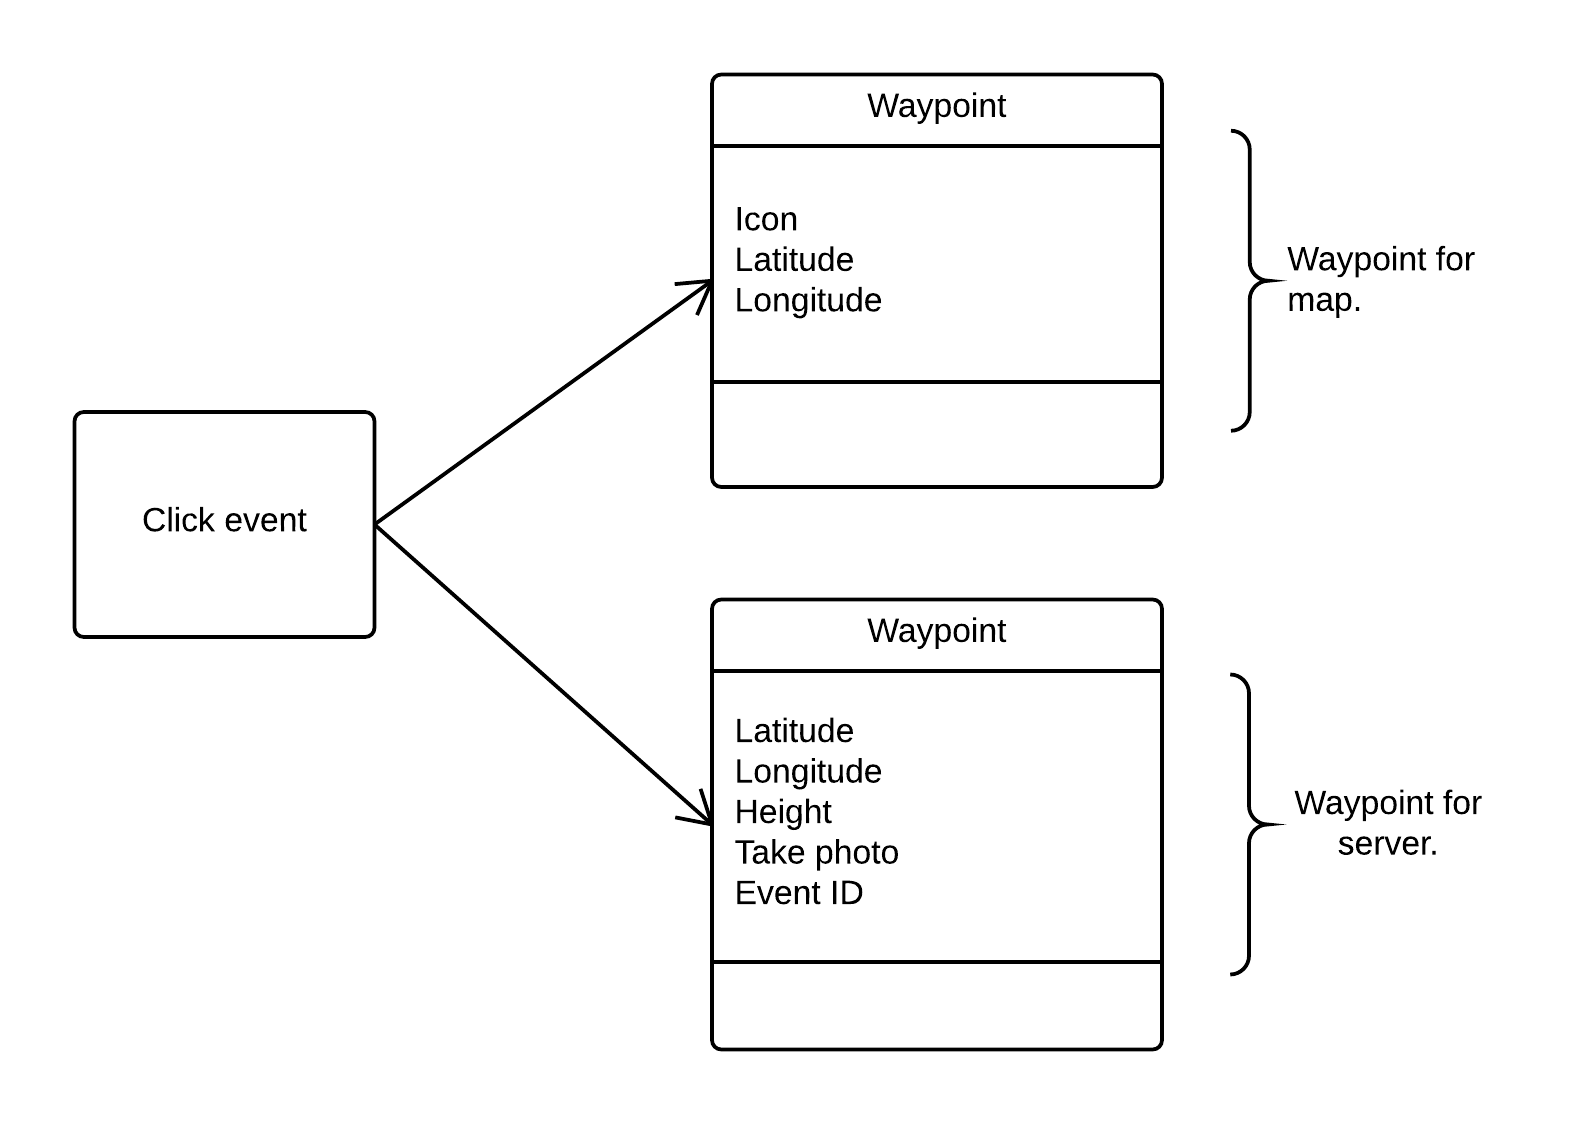
\includegraphics[width=0.6\textwidth]{Billeder/click_event.png}
	\vspace{-5pt}
	\caption{Click event eksempel}
	\label{fig:click_event}
\end{figure}